%----------------------------------------------------------------------------------------
%    PACKAGES AND THEMES
%----------------------------------------------------------------------------------------

\documentclass[aspectratio=169,xcolor=dvipsnames]{beamer}
\usetheme{SimpleDarkBlue}
\usepackage[UTF8]{ctex} % 主要中文支持包
\usepackage{fontspec}   % 字体设置
\usepackage{hyperref}
\usepackage{svg}
\svgsetup{
    inkscapeexe = D:/Inkspace/bin/inkscape.exe,
    inkscapelatex = false
}
\usepackage{graphicx} % Allows including images
\usepackage{booktabs} % Allows the use of \toprule, \midrule and \bottomrule in tables
\usepackage{tikz}
\usetikzlibrary{shapes,arrows,positioning}

\tikzstyle{block} = [rectangle, draw, rounded corners, minimum height=1.5cm, 
                    text width=3cm, text centered, drop shadow, fill=white]
%----------------------------------------------------------------------------------------
%    TITLE PAGE
%----------------------------------------------------------------------------------------

\title{Empathy in VR}

\author{The Sixth Group}

\date{\today} % Date, can be changed to a custom date

%----------------------------------------------------------------------------------------
%    PRESENTATION SLIDES
%----------------------------------------------------------------------------------------

\begin{document}

\begin{frame}
    \titlepage
\end{frame}

\begin{frame}{Overview}
    \tableofcontents
\end{frame}

% % First Teammate
% \section{Background}
\section{Background and Core Concept}
% --- 介绍两篇综述 ---
\begin{frame}{两篇关键系统性综述}
    背景部分汇报内容主要基于以下两篇近期的系统性综述论文:

    \begin{block}{Measurement of Empathy in Virtual Reality with Head-Mounted Displays: A Systematic Review\cite{lee2024measurement}}
        \textbf{期刊:} IEEE Transactions on Visualization and Computer Graphics \\
        \textbf{关注点:} HMD VR 对共情的影响;认知 vs. 情感共情;影响因素的\alert{元分析};强调VR作为认知共情工具。
    \end{block}

    \begin{block}{From Digital Media to Empathic Spaces: A Systematic Review of Empathy Research in Extended Reality Environments\cite{paananen2022digital}}
         \textbf{期刊:} ACM Computing Surveys \\
         \textbf{关注点:} 涵盖更广泛的 \alert{XR 环境};强调\alert{空间性 (Spatiality)} 的核心作用;提出“共情现实 (ER)”概念;关注设计伦理和未来研究路线图。
    \end{block}
\end{frame}
\begin{frame}{为何关注 VR 中的共情?}
    \begin{itemize}
        \item \textbf{共情的重要性:} 理解和感受他人情绪与处境的能力,是亲社会行为和人际连接的基础。
        \item \textbf{“终极共情机器”:} 虚拟现实 (VR) 提供前所未有的\alert{沉浸感}和\alert{临场感},允许用户“设身处地”体验他人视角,被 Chris Milk 等人誉为“终极共情机器”。
        \item \textbf{研究热点:} 随着 VR 技术(尤其是头戴式显示器 HMD)的普及,其在共情培养和研究中的应用日益受到关注。
    \end{itemize}
    \begin{figure}
        % 可以在此插入一张示意图,例如一个人戴着VR头显体验场景
        \includegraphics[width=0.6\linewidth]{background1.jpg}
        \caption{VR 提供沉浸式体验以促进共情}
    \end{figure}
\end{frame}

% --- 核心概念 ---
\begin{frame}{共情与 VR/XR}
    \begin{columns}[c]
        \column{.45\textwidth}
            \textbf{共情 (Empathy)}
            \begin{itemize}
                \item \textbf{认知共情 (Cognitive Empathy):} 理解他人观点、想法和意图的能力 (Perspective-taking)。
                \item \textbf{情感共情 (Emotional Empathy):} 分享和感受他人情绪状态的能力 (Affective response)。
                \item \textbf{其他维度:} 有时也提及躯体共情 (Somatic Empathy) 等。
            \end{itemize}

        \column{.45\textwidth}
            \textbf{虚拟/扩展现实 (VR/XR)}
             \begin{itemize}
                \item \textbf{VR:} 完全沉浸在计算机生成的虚拟世界中。
                \item \textbf{AR (增强现实):} 将数字信息叠加到现实世界。
                \item \textbf{MR (混合现实):} 虚拟与现实物体共存并可交互。
                \item \textbf{XR (扩展现实):} 涵盖 VR, AR, MR 的总称。
            \end{itemize}
    \end{columns}
     \begin{alertblock}{关键特性}
        VR/XR 的关键在于其\alert{沉浸性 (Immersion)}、\alert{临场感 (Presence)} 和 \alert{交互性 (Interactivity)},这些特性被认为有助于共情的产生。
    \end{alertblock}
\end{frame}

% --- 研究发现 (Lee et al.) ---
\begin{frame}{VR 对不同类型共情的影响}
    基于对 111 篇 HMD VR 研究的系统回顾与元分析 \cite{lee2024measurement}:
    \begin{block}{认知共情 vs. 情感共情}
        \begin{itemize}
            \item VR \alert{显著提升认知共情},该效果相对\alert{持久},不易随时间衰减。
            \item VR \alert{暂时提升情感共情},但效果会随时间推移\alert{回归基线水平}。
            \item VR 在提升认知共情方面\alert{优于 2D 视频},但在提升情感共情方面未显示明显优势(甚至可能不如2D视频)。
        \end{itemize}
    \end{block}
    \begin{theorem}[Lee et al. 结论推断]
       VR 可能更像是一个“终极\textbf{认知}共情机器”。它通过沉浸式视角转换,促进了对他人的理解,而非简单的情感传染。
    \end{theorem}
\end{frame}

\begin{frame}{影响 VR 共情效果的因素}
    \begin{columns}[t]
        \column{.48\textwidth}
            \textbf{显著影响因素 \cite{lee2024measurement}:}
             \begin{itemize}
                \item \textbf{年龄:} 对成年人和青年人的共情提升效果比儿童和青少年更显著。
                \item \textbf{国籍/文化:} 不同文化背景的参与者共情水平存在差异。
                \item \textbf{临场感 (Presence):} 与共情水平呈正相关。
                \item \textbf{具身感 (Embodiment):} 用户感觉自己拥有虚拟身体,与共情水平正相关。
                \item \textbf{叙事与故事性:} 可能比技术细节更重要。
            \end{itemize}

        \column{.48\textwidth}
             \textbf{影响不显著的因素:}
             \begin{itemize}
                \item \textbf{交互性 (Interactivity):} 主动交互 vs. 被动观看,在元分析中未发现对共情有显著影响。
                \item \textbf{共情目标 (Target of Empathy):} 针对自身、他人化身或环境,影响不显著。
                \item \textbf{视角 (Point of View):} 第一人称 vs. 第三人称等,影响不显著。
             \end{itemize}
            \begin{alertblock}{注意}
            这些因素影响不显著,是指在\textbf{荟萃分析统计层面}上。具体到单个实验或特定设计,它们可能仍有作用,尤其是叙事和角色塑造。
            \end{alertblock}
    \end{columns}
\end{frame}

% --- 研究发现 (Paananen et al.) ---
\begin{frame}{空间性在 XR 共情中的作用}
    基于对 XR 环境中共情研究的系统回顾:
    \begin{itemize}
        \item \textbf{空间性 (Spatiality) 是核心:} 人类通过空间理解世界,空间背景深刻影响共情体验。研究需关注共情发生的\alert{物理和虚拟空间环境}。
        \item \textbf{共情现实 (Empathic Reality, ER):} 在XR空间上叠加共情层,连接物理与虚拟,创造新的共情体验途径。
        \item \textbf{情境坍塌 (Context Collapse):} 现实世界的社会规范与虚拟世界的规则(或缺乏规则)可能发生冲突或融合,影响用户行为和共情。
        \item \textbf{非人类共情:} XR 可用于模拟非人类视角(动物、物体、自然现象),拓展共情的边界。
        \item \textbf{空间体验本身:} 安全感、可达性、美学等空间体验也可作为激发共情的来源(空间共情)。
    \end{itemize}
     \begin{examples}
        例如,在虚拟的贫民窟行走 \cite{paananen2022digital} 与在熟悉的办公室体验同事的困难,其空间背景带来的共情基础截然不同。
    \end{examples}
\end{frame}

% --- 测量与挑战 ---
\begin{frame}{如何测量 VR 中的共情?}
    \begin{columns}[c]
        \column{.5\textwidth}
            \textbf{常用方法:}
            \begin{itemize}
                \item \textbf{问卷调查 (最常用):}
                    \begin{itemize}
                        \item IRI (Interpersonal Reactivity Index)
                        \item BEA (Batson's Empathic Adjectives)
                        \item QCAE 等
                    \end{itemize}
                \item \textbf{生物信号:} EEG, HR, SCR 等 (研究较少)。
                \item \textbf{行为观察/分析。}
                \item \textbf{混合方法:} 结合定量与定性。
            \end{itemize}

        \column{.45\textwidth}
             \textbf{挑战与局限:}
             \begin{itemize}
                \item \textbf{主观性与偏见:} 问卷易受社会期许效应影响。
                \item \textbf{客观测量难度:} 生物信号数据处理复杂,与共情关联需验证。
                \item \textbf{长期效果追踪难:} 大部分研究只看短期效果。
                \item \textbf{生态效度:} 实验室环境与现实生活差异。
                \item \textbf{设计伦理:} 如何负责任地使用他人经验,避免伤害和刻板印象。
            \end{itemize}
    \end{columns}
    \begin{alertblock}{现状}
    当前测量仍以主观问卷为主,对共情的客观、长期、生态化测量是未来研究的重要方向。
    \end{alertblock}
\end{frame}


% --- 未来方向 ---
\begin{frame}{VR/XR 共情研究的未来展望}
    根据 \cite{paananen2022digital} 等综述的建议,未来研究可关注:
    \begin{itemize}
        \item \textbf{长期共情机制:} 探索如何设计能产生持久共情影响的XR体验。
        \item \textbf{超越人类的共情:} 研究如何利用XR促进对动物、自然环境甚至抽象概念的共情。
        \item \textbf{空间共情的深化:} 如何利用空间设计、空间叙事来增强共情?城市、家居等不同空间如何定制共情体验?
        \item \textbf{更鲁棒的测量与评估:} 发展更客观、结合情境的共情测量方法。
        \item \textbf{设计框架与伦理指南:} 建立XR共情工具的设计原则和伦理规范,平衡效果与责任。
        \item \textbf{元宇宙中的共情:} 在大规模、持续存在的虚拟世界中,共情将扮演何种角色?如何设计和管理?
    \end{itemize}
    \begin{examples}
        例如,开发一个持续性的AR应用,让用户在日常生活中通过空间线索感知城市无家可归者的困境,而非一次性的VR体验。
    \end{examples}
\end{frame}

% --- 结论 ---
\begin{frame}{总结}
    \begin{itemize}
        \item VR/XR 作为一种新兴媒介,在\alert{激发和研究共情}方面展现出巨大潜力,尤其是提升\alert{认知共情}。
        \item 其效果受到用户个人特征(年龄、文化)和体验设计(临场感、具身感、叙事)的影响,而交互方式等技术细节的直接影响可能相对较小。
        \item \alert{空间性(Spatiality)}是理解和设计XR共情体验的关键维度,需要超越传统媒介的视角。
        \item 当前研究在测量方法、长期效果、伦理规范等方面仍面临挑战。
        \item 未来的研究需要在深化理论理解、拓展应用场景(如非人类、空间共情)和完善设计实践(框架、伦理)方面继续努力。
    \end{itemize}
    \begin{alertblock}{核心信息}
    VR 不仅仅是技术,更是创造“体验”的工具。在共情领域,理解其如何塑造认知、情感和对空间的感知至关重要。
    \end{alertblock}
\end{frame}

\begin{frame}{References}
    \footnotesize
    \bibliography{reference.bib}
    \bibliographystyle{apalike}
\end{frame}

% Second Teammate
\section{Technology}
\begin{frame}{Technology}
    \centering
    \vspace{-0.5cm}
    
    \begin{columns}[onlytextwidth,T]
        \column{0.48\textwidth}
        \begin{block}{\color{white!80!black}存在性 }
 
        \end{block}
        
        \vspace{0.3cm}
        
        \begin{alertblock}{\color{white!70!black}具身VR和全身所有权错觉}

   
        \end{alertblock}
        
        \column{0.48\textwidth}
        \begin{block}{\color{white!80!black}代理错觉 }

 
        \end{block}
        
        \vspace{0.3cm}
        
        \begin{alertblock}{\color{white!80!black}内感知信号操控}


        \end{alertblock}
    \end{columns}
    
    \vspace{0.5cm}
    
    \begin{block}{\color{white!80!black}普罗透斯效应}
 

    \end{block}
    
    \vspace{0.3cm}
    
    \begin{beamercolorbox}[wd=0.9\textwidth,center,sep=4pt,rounded=true,shadow=true]{block body}
        \footnotesize
        这些技术相互配合,共同构建了一个能够促使用户产生共情和利他行为的虚拟环境。\\
        通过营造沉浸感、建立身体所有权、增强代理感、调节情绪以及引导行为,\\
        VR技术展现了其在促进共情能力方面的巨大潜力。
    \end{beamercolorbox}
\end{frame}


\begin{frame}{存在性}
    \begin{enumerate}
        \item 存在性:通过地方错觉和可信度错觉,VR可以让用户感受到身临其境和真实,从而更容易产生共情。
        \begin{itemize}
            \item \textbf{存在性 (Presence):}
            \item 地方错觉 (Place Illusion): 通过高分辨率、大视场角的显示技术,结合3D音频和触觉反馈(如触觉手套、振动平台),营造出身临其境的虚拟环境,让用户感觉像真的置身于虚拟场景中。
            \item 可信度错觉 (Plausibility Illusion): 通过逼真的图形渲染、物理引擎模拟、以及符合现实世界逻辑的交互设计,让虚拟环境的行为和反应看起来真实可信,增强用户的沉浸感。
        \end{itemize}
    \end{enumerate}
\end{frame}

\begin{frame}{具身VR和全身所有权错觉}
    \begin{enumerate}
        \setcounter{enumi}{1}
        \item 具身VR和全身所有权错觉:通过让用户感受到自己拥有一个不同的身体,VR可以让用户从他人视角体验世界,从而更容易理解他人的感受和需求。
        \begin{itemize}
            \item \textbf{具身VR和全身所有权错觉 (Embodiment and Body Ownership Illusion):}
            \item 具身VR (Embodied VR): 使用能够追踪全身动作的传感器(如全身动捕系统、深度摄像头),将用户的动作实时映射到虚拟化身上,使用户能够以虚拟身体的视角在虚拟环境中进行交互。
            \item 全身所有权错觉 (Body Ownership Illusion): 通过视觉、触觉和本体感觉的同步,让用户将虚拟身体感知为自己的身体。例如,当虚拟手接触虚拟物体时,用户的手也同时感受到触觉反馈,从而增强对虚拟身体的拥有感。
        \end{itemize}
    \end{enumerate}
\end{frame}

\begin{frame}{代理错觉}
    \begin{enumerate}
        \setcounter{enumi}{2}
        \item 代理错觉:通过让用户感受到自己对虚拟身体的行动具有控制权,VR可以让用户产生对利他行为的自我归因,从而增强利他行为。
        \begin{itemize}
            \item \textbf{代理错觉 (Agency):}
            \item 动作同步 (Action Synchronization): 精确的动作捕捉和低延迟的渲染技术,确保用户的动作与虚拟化身的行为同步,让用户感觉自己完全控制着虚拟身体。
            \item 因果反馈 (Causal Feedback): 虚拟环境对用户的动作做出符合预期的反应,例如,虚拟手按下按钮后,虚拟设备启动,使用户明确感知到自己的行为对环境产生了影响。
        \end{itemize}
    \end{enumerate}
\end{frame}

\begin{frame}{内感知信号操控}
    \begin{enumerate}
        \setcounter{enumi}{3}
        \item 内感知信号操控:通过操控用户的生理信号,VR可以帮助用户控制情绪,从而将共情转化为同情和利他行为。
        \begin{itemize}
            \item \textbf{内感知信号操控 (Interoceptive Signal Manipulation):}
            \item 生理信号监测 (Physiological Signal Monitoring): 使用生物传感器(如心率监测仪、呼吸传感器、皮肤电传感器)实时监测用户的生理状态。
            \item 生理信号反馈 (Physiological Signal Feedback): 将监测到的生理信号以视觉、听觉或触觉的形式反馈给用户,例如,将心率以虚拟场景中的颜色变化表示,或者通过调整虚拟环境的音乐节奏来反映用户的情绪状态。
            \item 生理信号调节 (Physiological Signal Regulation): 通过生物反馈技术,引导用户调节自己的生理状态,例如,通过控制呼吸来降低心率,从而控制情绪。
        \end{itemize}
    \end{enumerate}
\end{frame}

\begin{frame}{普罗透斯效应}
    \begin{enumerate}
        \setcounter{enumi}{4}
        \item 普罗透斯效应:通过使用具有利他特征的虚拟形象,VR可以影响用户的行为和态度,从而促进共情和利他行为。
        \begin{itemize}
            \item \textbf{普罗透斯效应 (Proteus Effect):}
            \item 虚拟化身定制 (Avatar Customization): 允许用户自定义虚拟化身的外貌、性格和行为特征,特别是赋予其具有利他特征的属性,如帮助他人的行为、友善的表情等。
            \item 行为引导 (Behavioral Priming): 在虚拟环境中设计特定的情境和任务,引导用户扮演具有利他特征的虚拟角色,例如,帮助虚拟角色解决困难、与虚拟角色进行积极的互动等。
        \end{itemize}
    \end{enumerate}
    
    \vspace{5mm}
    
\end{frame}
 \begin{frame}{设计基于VR的共情训练的框架 }
    该框架基于三个关键问题,并提供了相关的共情能力、调节器、催化剂、学习方法和VR技术。旨在帮助教育者设计有效的VR共情训练应用。
     \begin{block}{What is the relationship between emote and observer?}
        情绪化者与观察者之间的关系是什么?
     \end{block}

     \begin{alertblock}{How developed is the self-awareness of the observer?}
     观察者的自我意识是如何发展的?
      \end{alertblock}

     \begin{block}{How developed are the empathic abilities of the observer toward the emote?}
     观察者对情绪化者的同理心能力如何发展?
      \end{block}
     
          
 \end{frame}
 
\begin{frame}{What is the relationship between emote and observer?}
    
    \begin{enumerate}
        \item \textbf{What is the relationship between emote and observer?(情绪化者与观察者之间的关系是什么?)}
        \begin{itemize}
            \item Abilities(能力):群际开放性、反思思维、社交技能、冲突管理。
            \item Catalysts(催化剂):长期培训、安全环境、协作动力、参与志愿活动。
            \item Moderators(调节器):增加对外群体成员的熟悉度、亲和力和相似性;减少偏见、刻板印象、编码预测和对内群体成员的分类思考;增强平等主义目标和自我分析。
            \item Learning methods(学习方法):建构主义和社会情感学习用于反思思维的仪器化;实施平等主义目标;重复启动非刻板印象联想;个体化和否定刻板印象;正念训练用于非评判性思维实践。
            \item EVR methods(虚拟现实方法):增强自我-其他相似性的群体间体现;普罗透斯效应
        \end{itemize}
    \end{enumerate}
\end{frame}

\begin{frame}{How developed is the self-awareness of the observer?}
    \begin{enumerate}
        \setcounter{enumi}{1}
        \item \textbf{How developed is the self-awareness of the observer?(观察者的自我意识是如何发展的?)}
        \begin{itemize}
            \item Abilities(能力):身体、情感、认知和社会自我意识。
            \item Catalysts(催化剂):教育者作为促进者。
            \item Moderators(调节器):自我-他人区分;情绪识别;平等主义的内部和社会目标。
            \item Learning methods(学习方法):正念训练用于内省觉知;实施平等主义目标;心理扫描。
            \item EVR methods(虚拟现实方法):PI和PSI错觉;内感知信号操控。
        \end{itemize}
    \end{enumerate}
\end{frame}

\begin{frame}{How developed are the empathic abilities of the observer toward the emote?}
    \begin{enumerate}
        \setcounter{enumi}{2}
        \item \textbf{How developed are the empathic abilities of the observer toward the emote?(观察者对情绪化者的同理心能力如何发展?)}
        \begin{itemize}
            \item Abilities(能力):情感同理心、认知同理心、同理心准确性、同理心痛苦调节、同情心、利他主义、问题解决。
            \item Catalysts(催化剂):基于真实世界的案例和情境知识。
            \item Moderators(调节器):情感投入、视角转换、在线模拟、对话技巧、当前注意力、仁爱、动机、帮助的力量和技巧;行为表达的自控。
            \item Learning methods(学习方法):角色扮演;正念训练用于当前注意力、视角转换和同情心;实施平等主义目标;心理扫描。
            \item EVR methods(虚拟现实方法):多传感器第一人称视角转换同步性;普罗透斯效应和代理错觉。
        \end{itemize}
    \end{enumerate}
\end{frame}

% % Third Teammate
% \section{Applications}

% % Fourth Teammate
% \section{Evaluation}

% % Fifth Teammate
% \section{Challenges}
% \begin{frame}{Challenges}
    
% \end{frame}

\begin{frame}
    \begin{center}
        \textit{This page is intentionally left blank.}
    \end{center}
\end{frame}

% 第四部分
%------------------------------------------------
\section{Introduction}
%------------------------------------------------

\begin{frame}{The "Empathy Machine" Hypothesis}
    \begin{itemize}
        \item VR被誉为「终极共情机器」,但缺乏实证支持
        \item \alert{核心问题}:如何将VR特性与共情结果关联?
        \item \textbf{共情类型}:
            \begin{itemize}
                \item 认知共情:理解他人视角(如叙事驱动)
                \item 情感共情:情感共鸣(如身体反应)
            \end{itemize}
    \end{itemize}
    \begin{block}{研究目标}
        开发轻量级协议,低成本捕捉VR中的共情数据
    \end{block}
\end{frame}

%------------------------------------------------
\section{Challenges}
%------------------------------------------------

\begin{frame}{测量VR共情的挑战}
    \begin{columns}[t]
        \column{.5\textwidth}
        \textbf{方法论局限}
        \begin{itemize}
            \item 自我报告的偏差(记忆衰减/认知过载)
            \item 生理监测成本高(心率/皮肤电导)
            \item VR特有因素:沉浸感、具身性、临场感
        \end{itemize}
        
        \column{.5\textwidth}
        \textbf{技术挑战}
        \begin{itemize}
            \item 第一人称视角难以外部观察
            \item 玩家操作学习曲线干扰情感数据
            \item 标准化工具的缺乏
        \end{itemize}
    \end{columns}
\end{frame}

%------------------------------------------------
\section{Proposed Framework}
%------------------------------------------------

\begin{frame}{轻量级测量协议}
    \begin{block}{核心设计原则}
        \begin{itemize}
            \item 低成本:仅需基础VR设备 + 免费软件(OBS Studio)
            \item 多模态数据:同步录制玩家动作 + VR画面 + 音频
            \item 标准化工具:情感轮 + IOS量表
        \end{itemize}
    \end{block}
    
    \begin{figure}
        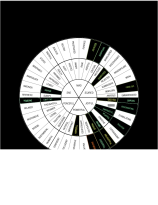
\includegraphics[width=0.3\linewidth]{g1434.pdf}  % 需替换为实际图片
        \caption{情感轮(Plutchik, 1980)}
    \end{figure}
\end{frame}

%------------------------------------------------

\begin{frame}{实验流程设计}
    \begin{columns}[c]
        \column{.6\textwidth}
        \begin{enumerate}
            \item \textbf{预访谈}:评估VR熟悉度
            \item \textbf{第一次体验}(20分钟):熟悉操作
            \item \textbf{视频回放访谈}:情感轮标记关键瞬间
            \item \textbf{第二次体验}(30分钟):聚焦叙事
            \item \textbf{后测问卷}:VR版IOS量表
        \end{enumerate}
        
        \column{.4\textwidth}
        \begin{alertblock}{关键创新}
            多次体验减少操作干扰,增强叙事沉浸
        \end{alertblock}
    \end{columns}
\end{frame}

%------------------------------------------------
\section{Key Findings}
%------------------------------------------------

\begin{frame}{实验结果}
    \begin{itemize}
        \item \textbf{身体反应的价值}:姿势变化/无意识言语揭示共情强度
        \item \textbf{玩家熟悉度}:新手因操作挫折降低共情得分(需基线校准)
        \item \textbf{重复体验效应}:第二次体验的叙事共情提升40\%(示例数据)
    \end{itemize}
    
    \begin{exampleblock}{典型反馈}
        「第二次体验时,我更关注角色的手势细节,感受到更强的代入感」
    \end{exampleblock}
\end{frame}

%------------------------------------------------
\section{Limitations \& Future Work}
%------------------------------------------------

\begin{frame}{局限与未来方向}
    \begin{columns}[t]
        \column{.5\textwidth}
        \textbf{当前局限}
        \begin{itemize}
            \item 工具验证不足(如情感轮 vs. EQ量表)
            \item 缺乏共情基线数据
            \item 样本局限于研究团队
        \end{itemize}
        
        \column{.5\textwidth}
        \textbf{未来计划}
        \begin{itemize}
            \item 跨群体验证协议鲁棒性
            \item 集成实时生理监测(低成本方案)
            \item 开发自动化情感标注工具
        \end{itemize}
    \end{columns}
\end{frame}

%------------------------------------------------
\section{Conclusion}
%------------------------------------------------

\begin{frame}{研究意义}
    \begin{itemize}
        \item \alert{方法论贡献}:首个针对VR共情的轻量级标准化协议
        \item \textbf{设计启示}:通过重复体验优化叙事沉浸
        \item \textbf{跨学科潜力}:支持心理学、HCI、游戏设计的共情研究
    \end{itemize}
    
    \begin{block}{愿景}
        推动「共情驱动型VR」从概念到实证的转化
    \end{block}
\end{frame}

%------------------------------------------------

\begin{frame}
    \begin{center}
        \textit{This page is intentionally left blank.}
    \end{center}
\end{frame}


\begin{frame}
\frametitle{Ethical Challenges \& Future Directions}
\begin{itemize}
    \item \textbf{VR as the “Ultimate Empathy Machine”:}
    \begin{itemize}
        \item Virtual Reality (VR) has been promoted as a tool to foster empathy, especially for social and humanitarian causes (e.g., refugee crises, racial issues).
        \item Industry claims that VR enhances empathy more effectively than traditional media by providing immersive, embodied experiences.
    \end{itemize}
    \item \textbf{Critical Review:}
    \begin{itemize}
        \item This paper critiques the "VR-empathy" model, arguing that there is insufficient evidence to support VR's universal ability to enhance empathy in the long term.
    \end{itemize}
\end{itemize}
\end{frame}

\begin{frame}
\frametitle{The VR-Empathy Model and Its Issues}
\begin{itemize}
    \item \textbf{Claim of Empathy through Immersion:}
    \begin{itemize}
          \item VR aims to elicit empathy by allowing users to experience another person’s life firsthand (e.g., VR films like \textit{Clouds Over Sidra}). For more details, visit the following link: \href{https://v.qq.com/x/page/d03194nt7hs.html}{Click here to watch}.

        \item Proponents claim that VR fosters pro-social behavior by connecting people emotionally with others' experiences.
    \end{itemize}
    \item \textbf{Empirical Challenges:}
    \begin{itemize}
        \item \textbf{Lack of Evidence:} Studies show mixed results; no substantial proof that VR leads to long-term empathy or motivates pro-social behavior.
        \item \textbf{Bias and Short-Term Effects:} Responses are often influenced by personal biases (e.g., race, gender) and may be short-lived.
    \end{itemize}
\end{itemize}
\end{frame}

\begin{frame}
\frametitle{Key Findings from Empirical Studies}
\begin{itemize}
    \item \textbf{Lack of Long-Term Effects:}
    \begin{itemize}
        \item \textbf{Studies:} Few long-term studies on the impact of VR on empathy, with most studies showing only short-term changes in attitudes.
        \item \textbf{Comparison to Other Media:} Other media (cinema, literature) may be just as effective in fostering empathy.
    \end{itemize}
    \item \textbf{Cultural and Personal Biases:}
    \begin{itemize}
        \item \textbf{Impact of Identity:} Participants’ empathy is influenced by their own social identity and biases, which can distort the effectiveness of VR empathy experiences.
        \item \textbf{Empathy for Similar Groups:} People often feel more empathy for individuals they perceive as similar to themselves (e.g., same race, gender).
    \end{itemize}
\end{itemize}
\end{frame}

\begin{frame}
\frametitle{Ethical Considerations in VR Empathy}
\begin{itemize}
    \item \textbf{Mediated Empathy and Ethical Concerns:}
    \begin{itemize}
        \item VR experiences may induce “empathetic stress,” causing emotional fatigue or discomfort, particularly in vulnerable groups.
        \item \textbf{Risk of Exploitation:} The voyeuristic nature of some VR experiences may objectify those portrayed, creating a false sense of empathy or detachment.
    \end{itemize}
    \item \textbf{Need for Ethical Guidelines:}
    \begin{itemize}
        \item Ethical concerns include audience safety, emotional well-being, and ensuring that VR content is responsibly designed, especially when dealing with sensitive topics.
    \end{itemize}
\end{itemize}
\end{frame}

\begin{frame}
\frametitle{Future Research Directions}
\begin{itemize}
    \item \textbf{Need for Rigorous Research:}
    \begin{itemize}
        \item \textbf{Longitudinal Studies:} More long-term studies are required to assess the lasting impact of VR on empathy.
        \item \textbf{Cultural Sensitivity:} Research should consider how VR experiences are received by different cultural groups and how personal biases affect empathy responses.
    \end{itemize}
    \item \textbf{Design Considerations:}
    \begin{itemize}
        \item VR experiences should not just focus on immersion and empathy but also integrate critical thinking and reflection about the social issues depicted.
        \item Storytelling elements and interactive designs should be carefully crafted to encourage meaningful engagement and empathy.
    \end{itemize}
\end{itemize}
\end{frame}

\begin{frame}
\frametitle{Conclusion}
\begin{itemize}
    \item \textbf{VR’s Potential vs. Reality:}
    \begin{itemize}
        \item While VR has potential to foster empathy, it should not be viewed as a "magic bullet" for social change.
        \item There is insufficient evidence to claim VR as an inherently superior medium for empathy compared to traditional media.
    \end{itemize}
    \item \textbf{Call for More Research:}
    \begin{itemize}
        \item Future studies must rigorously evaluate the long-term effects of VR and develop ethical frameworks for its use in social and humanitarian contexts.
    \end{itemize}
\end{itemize}
\end{frame}

\begin{frame}
\frametitle{Questions}
\begin{itemize}
    \item Thank you for your attention!  
    \item Feel free to ask any questions.
\end{itemize}
\end{frame}

\end{document}
\end{document}

% %------------------------------------------------
% \section{First Section}
% %------------------------------------------------

% \begin{frame}{Bullet Points}
%     \begin{itemize}
%         \item Lorem ipsum dolor sit amet, consectetur adipiscing elit
%         \item Aliquam blandit faucibus nisi, sit amet dapibus enim tempus eu
%         \item Nulla commodo, erat quis gravida posuere, elit lacus lobortis est, quis porttitor odio mauris at libero
%         \item Nam cursus est eget velit posuere pellentesque
%         \item Vestibulum faucibus velit a augue condimentum quis convallis nulla gravida
%     \end{itemize}
% \end{frame}

% %------------------------------------------------

% \begin{frame}{Blocks of Highlighted Text}
%     In this slide, some important text will be \alert{highlighted} because it's important. Please, don't abuse it.

%     \begin{block}{Block}
%         Sample text
%     \end{block}

%     \begin{alertblock}{Alertblock}
%         Sample text in red box
%     \end{alertblock}

%     \begin{examples}
%         Sample text in green box. The title of the block is ``Examples".
%     \end{examples}
% \end{frame}

% %------------------------------------------------

% \begin{frame}{Multiple Columns}
%     \begin{columns}[c] % The "c" option specifies centered vertical alignment while the "t" option is used for top vertical alignment

%         \column{.45\textwidth} % Left column and width
%         \textbf{Heading}
%         \begin{enumerate}
%             \item Statement
%             \item Explanation
%             \item Example
%         \end{enumerate}

%         \column{.45\textwidth} % Right column and width
%         Lorem ipsum dolor sit amet, consectetur adipiscing elit. Integer lectus nisl, ultricies in feugiat rutrum, porttitor sit amet augue. Aliquam ut tortor mauris. Sed volutpat ante purus, quis accumsan dolor.

%     \end{columns}
% \end{frame}

% %------------------------------------------------
% \section{Second Section}
% %------------------------------------------------

% \begin{frame}{Table}
%     \begin{table}
%         \begin{tabular}{l l l}
%             \toprule
%             \textbf{Treatments} & \textbf{Response 1} & \textbf{Response 2} \\
%             \midrule
%             Treatment 1         & 0.0003262           & 0.562               \\
%             Treatment 2         & 0.0015681           & 0.910               \\
%             Treatment 3         & 0.0009271           & 0.296               \\
%             \bottomrule
%         \end{tabular}
%         \caption{Table caption}
%     \end{table}
% \end{frame}

% %------------------------------------------------

% \begin{frame}{Theorem}
%     \begin{theorem}[Mass--energy equivalence]
%         $E = mc^2$
%     \end{theorem}
% \end{frame}

% %------------------------------------------------

% \begin{frame}{Figure}
%     Uncomment the code on this slide to include your own image from the same directory as the template .TeX file.
%     %\begin{figure}
%     %\includegraphics[width=0.8\linewidth]{test}
%     %\end{figure}
% \end{frame}

% %------------------------------------------------

% \begin{frame}[fragile] % Need to use the fragile option when verbatim is used in the slide
%     \frametitle{Citation}
%     An example of the \verb|\cite| command to cite within the presentation:\\~

%     This statement requires citation \cite{p1}.
% \end{frame}

% %------------------------------------------------

% \begin{frame}{References}
%     \footnotesize
%     \bibliography{reference.bib}
%     \bibliographystyle{apalike}
% \end{frame}

% %------------------------------------------------

% \begin{frame}
%     \Huge{\centerline{\textbf{The End}}}
% \end{frame}

% %----------------------------------------------------------------------------------------
